\section{Results}

\begin{frame}[shrink=5]{Local Reproduction: CC GENERAL}
    \begin{columns}[T,onlytextwidth]
        \begin{column}{0.4\textwidth}
            \small
            \begin{beamercolorbox}[sep=0.7em, rounded=true, shadow=true]{block title}
                \textbf{Setup}
            \end{beamercolorbox}
            \vspace{0.1cm}
            \begin{itemize}
                \item 8,950 customers
                \item 17 numeric features
                \item injected missingness \(\approx 30\%\)
                \item KMeans init + alternating GMM updates
            \end{itemize}

            \vspace{0.2cm}
            \begin{beamercolorbox}[sep=0.6em, rounded=true, shadow=true]{block body}
                \textbf{Observed run}\\
                convergence after \textbf{199} iterations\\
                silhouette score \textbf{0.1489}
            \end{beamercolorbox}
        \end{column}
        \begin{column}{0.56\textwidth}
            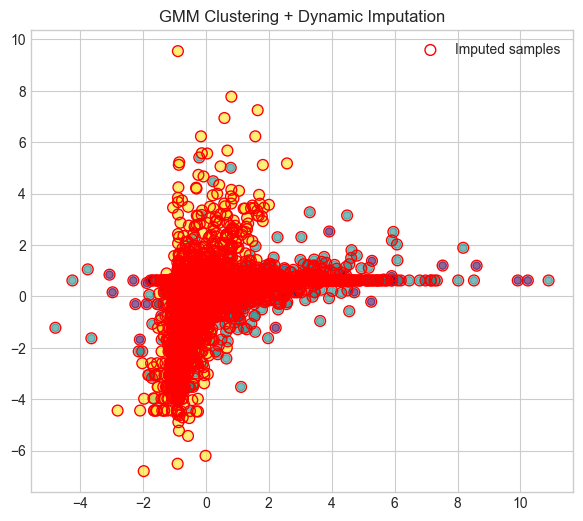
\includegraphics[width=\textwidth]{../latex_report/figures/notebook_exports/GMM_Nhat_cell8_out1.png}
        \end{column}
    \end{columns}
\end{frame}


\begin{frame}[shrink=3]{Application Case: Airplane Crashes}
    \begin{columns}[T,onlytextwidth]
        \begin{column}{0.34\textwidth}
            \begin{beamercolorbox}[sep=0.8em, rounded=true, shadow=true]{block title}
                \textbf{Pipeline}
            \end{beamercolorbox}
            \begin{itemize}
                \item 5,236 usable rows
                \item 6 numeric features
                \item MCAR masking at \(20\%\)
                \item \(\scal{K}=4\) Gaussian components
            \end{itemize}

            \vspace{0.2cm}
            \begin{beamercolorbox}[sep=0.7em, rounded=true, shadow=true]{alerted text}
                RMSE on masked entries\\
                {\LARGE \textbf{20.0588}}
            \end{beamercolorbox}
        \end{column}
        \begin{column}{0.62\textwidth}
            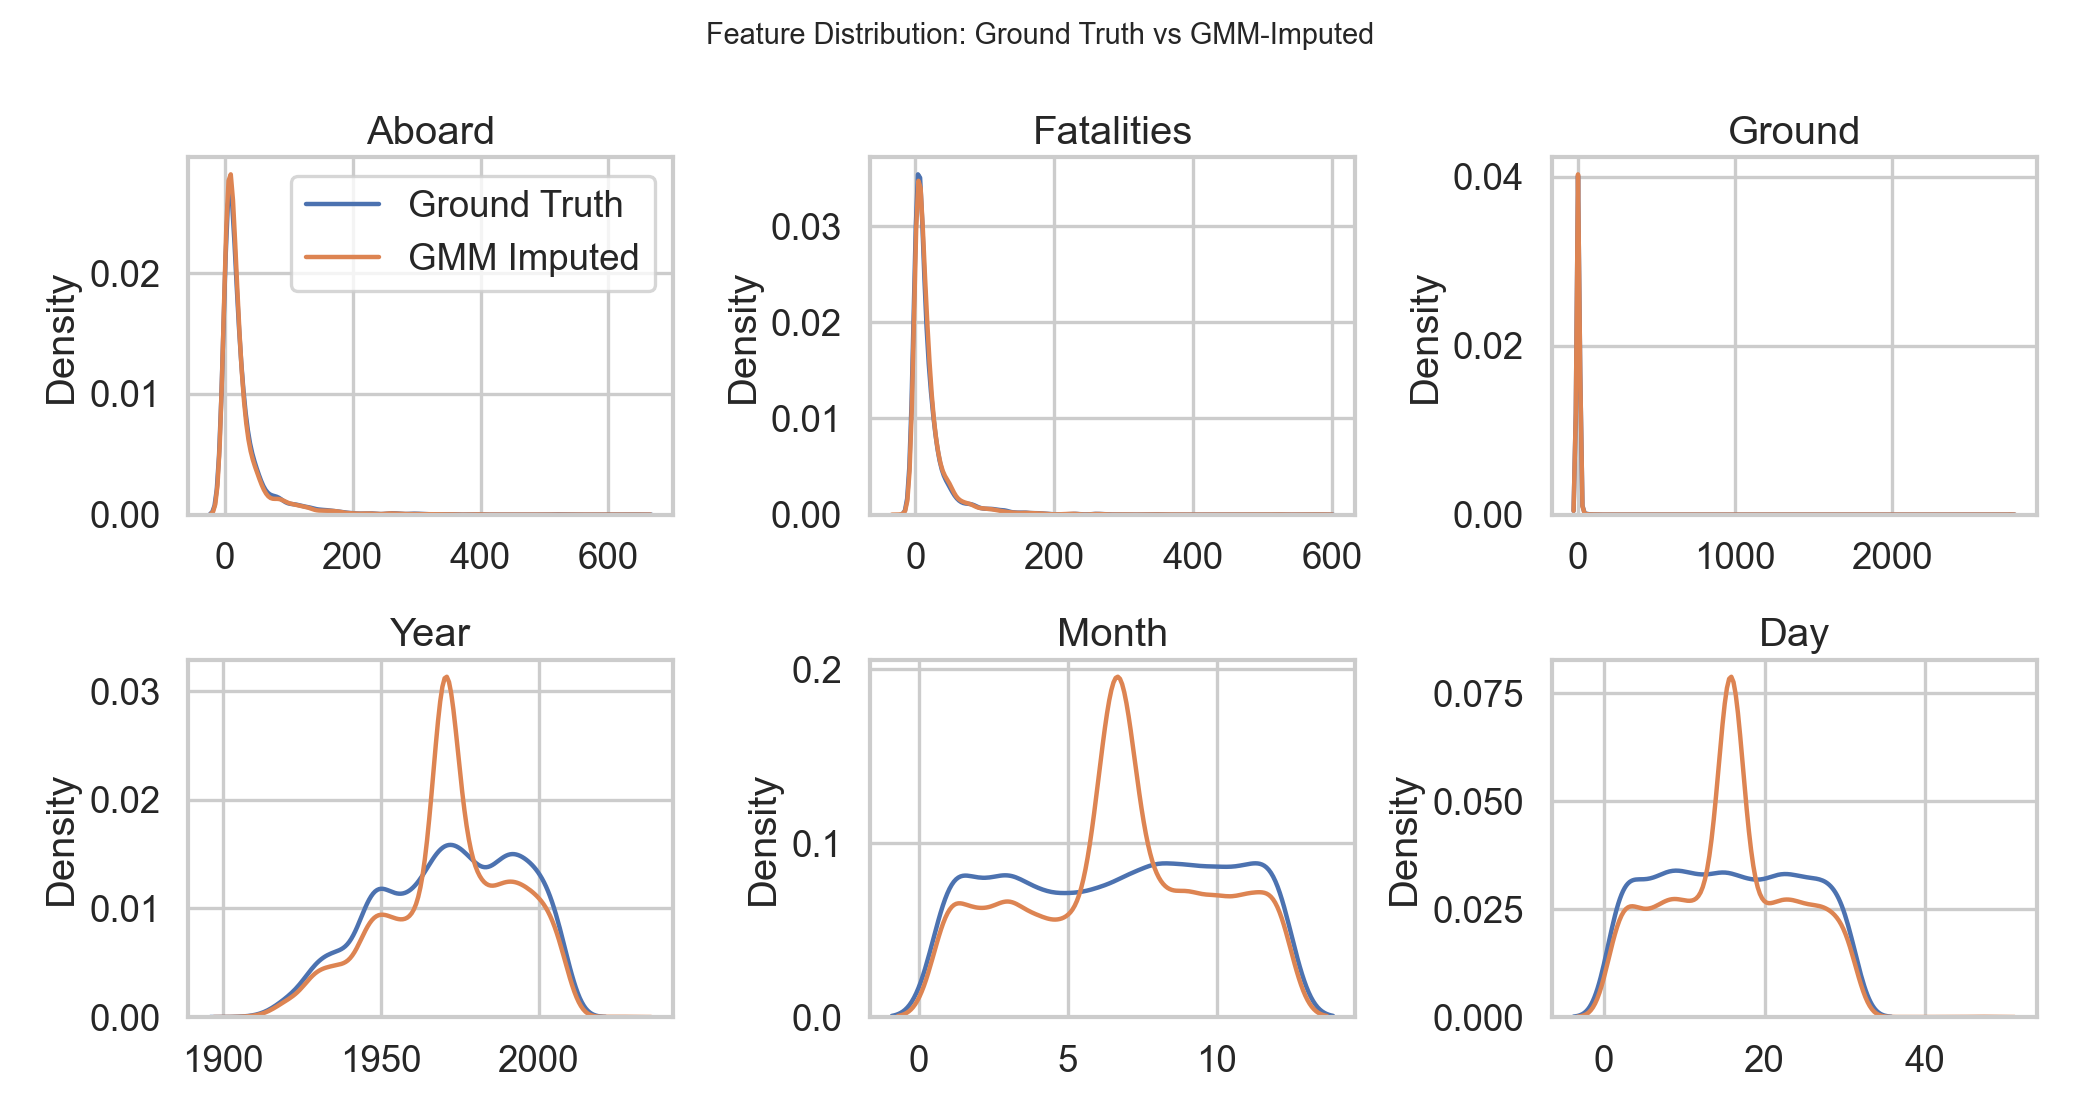
\includegraphics[width=\textwidth]{../latex_report/figures/applications/distribution_comparison.png}
        \end{column}
    \end{columns}
\end{frame}


\begin{frame}[shrink=10]{What the Visual Artifacts Say}
    \begin{columns}[T,onlytextwidth]
        \begin{column}{0.48\textwidth}
            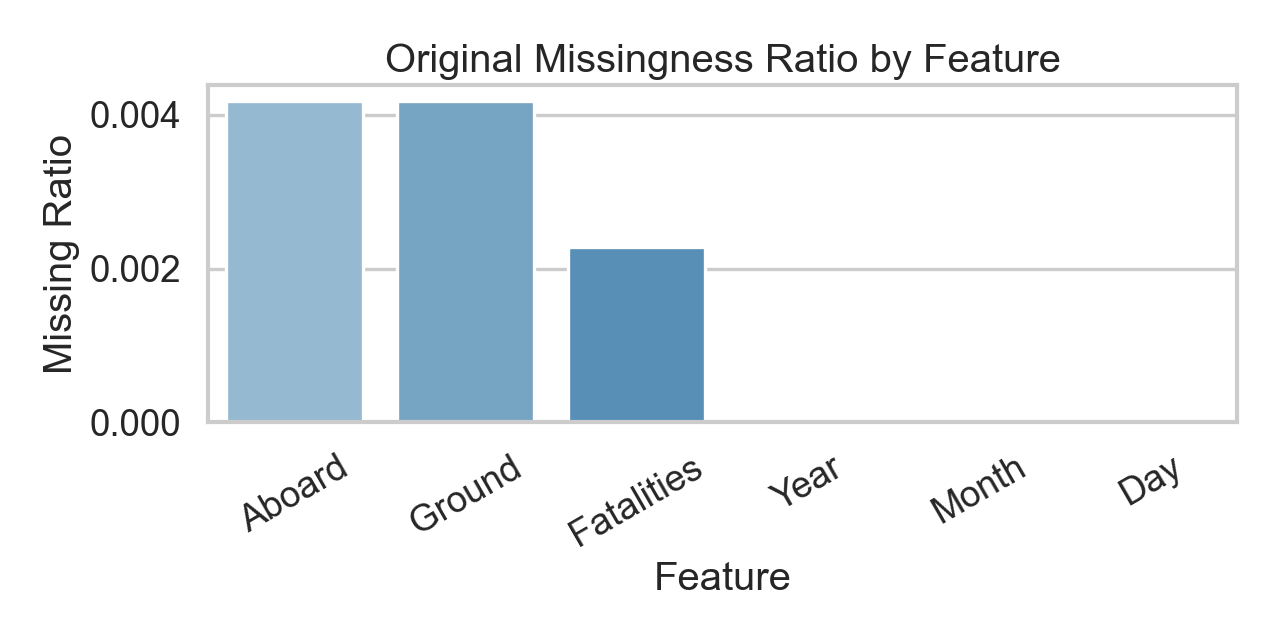
\includegraphics[width=\textwidth]{../latex_report/figures/applications/missingness_ratio.png}
            \vspace{0.1cm}
            \begin{center}
                \small feature-level missingness profile
            \end{center}
        \end{column}
        \begin{column}{0.48\textwidth}
            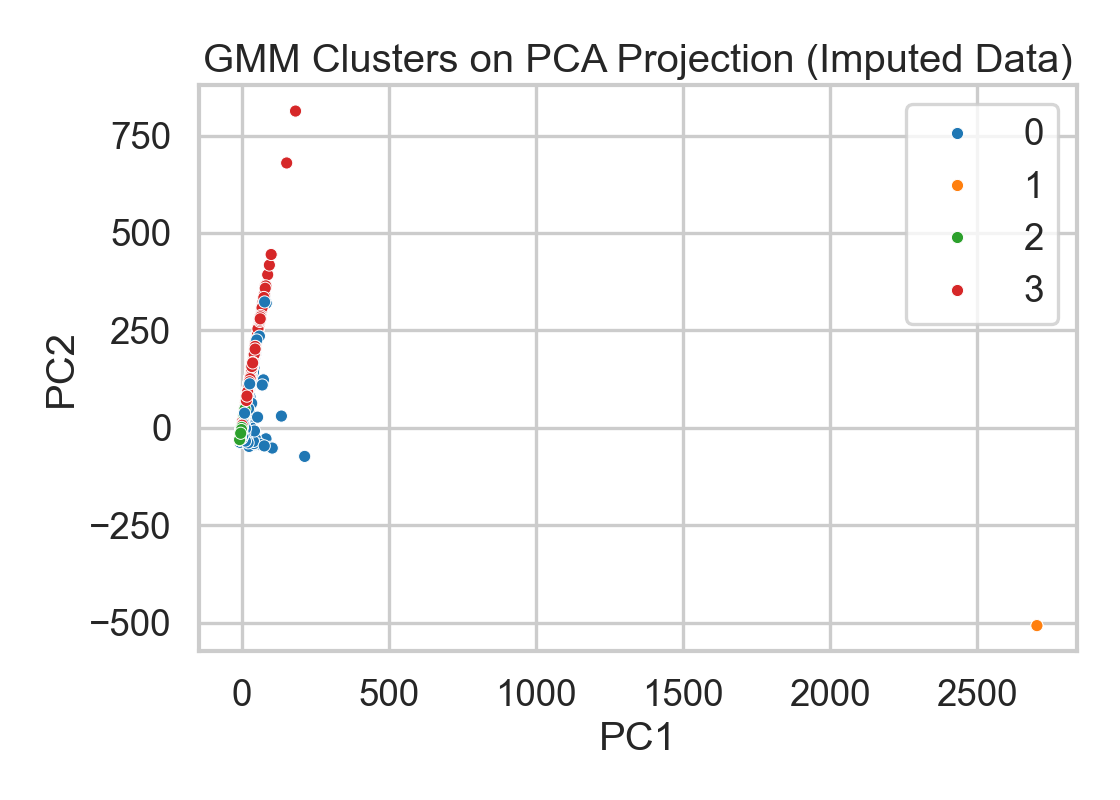
\includegraphics[width=\textwidth]{../latex_report/figures/applications/pca_clusters.png}
            \vspace{0.1cm}
            \begin{center}
                \small geometry after dynamic imputation
            \end{center}
        \end{column}
    \end{columns}

    \vspace{0.25cm}
    \begin{center}
        \large
        \textbf{The method is not only mathematically elegant.}\\
        It survives contact with real, dirty tabular data.
    \end{center}
\end{frame}
